\section{Experiments}
\label{sec:experiments}

\begin{figure}[t!]
\begin{center}
%\includegraphics[width=0.75\textwidth]{figs/sketch-comparison.png}
\begin{arxiv}
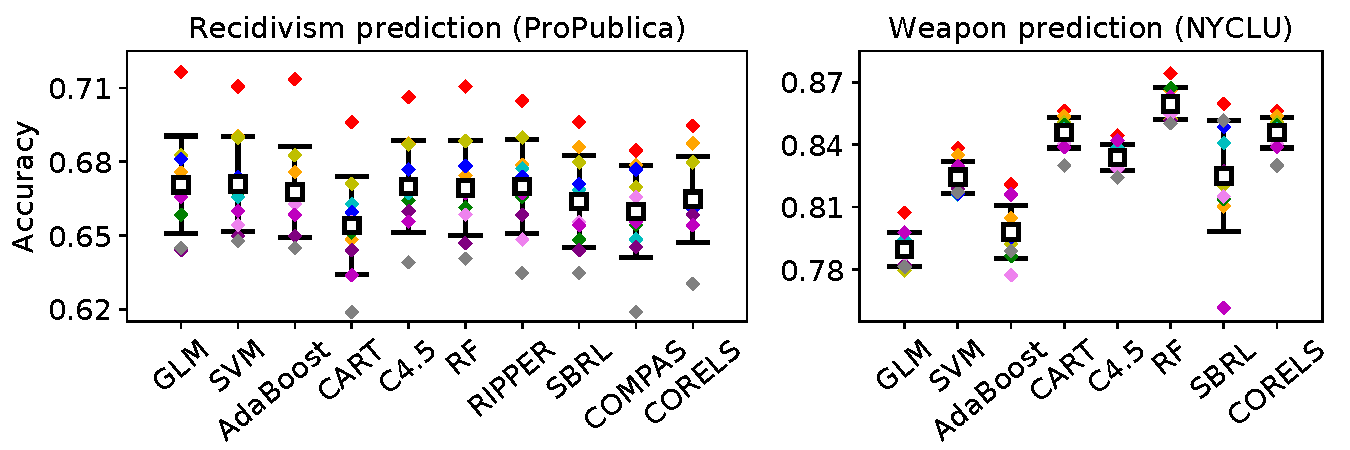
\includegraphics[trim={10mm, 5mm, 25mm, 5mm},
width=\textwidth]{figs/compare-compas-weapon.pdf}
\end{arxiv}
\begin{kdd}
% left lower right upper
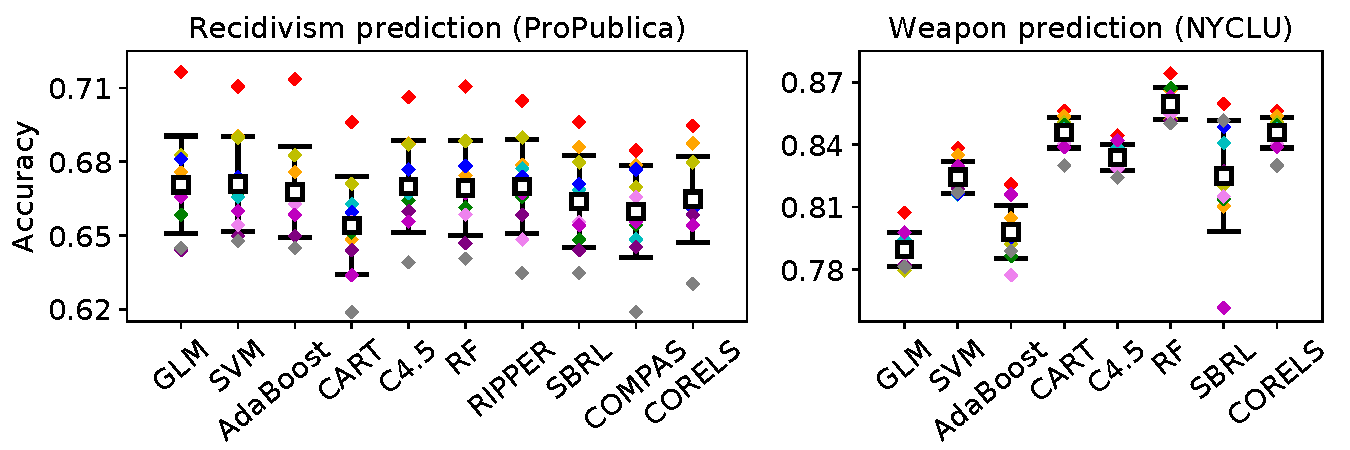
\includegraphics[trim={10mm, 11mm, 25mm, 5mm},
width=0.48\textwidth]{figs/compare-compas-weapon.pdf}
\end{kdd}
\end{center}
\caption{Test accuracy means (white squares),
standard deviations (error bars),
and values (colors correspond to folds).
}
\label{fig:comparison}
\end{figure}

\begin{figure}[t!]
\begin{center}
%\includegraphics[width=0.75\textwidth]{figs/sketch-comparison.png}
\begin{arxiv}
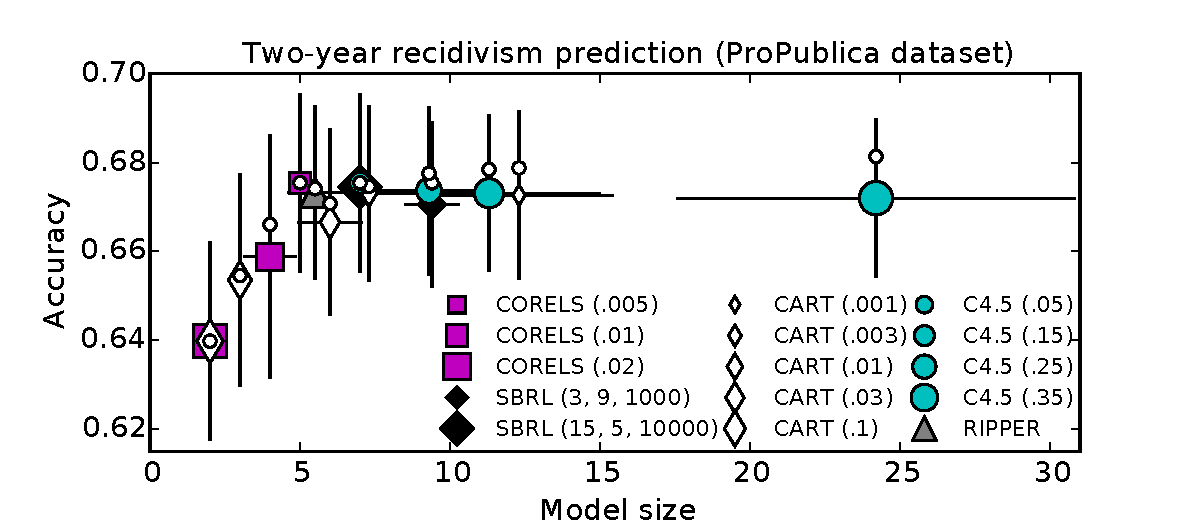
\includegraphics[trim={12mm, 0mm, 24mm, 5mm},
width=0.75\textwidth]{figs/compas-sparsity-training.pdf}
\end{arxiv}
\begin{kdd}
% left lower right upper
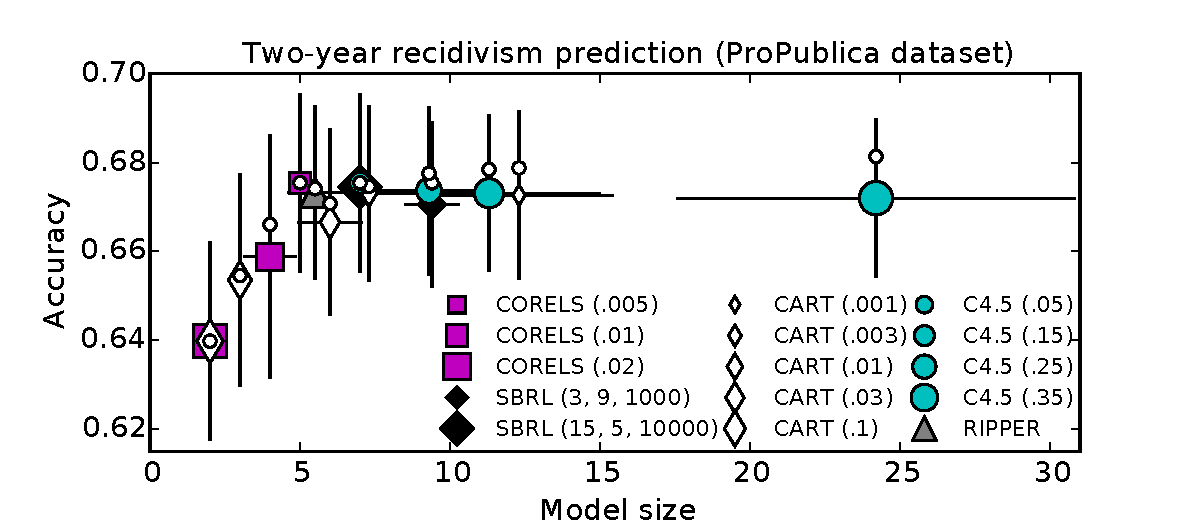
\includegraphics[trim={12mm, 0mm, 24mm, 5mm}, width=0.43\textwidth]{figs/compas-sparsity-training.pdf}
\end{kdd}
\begin{arxiv}
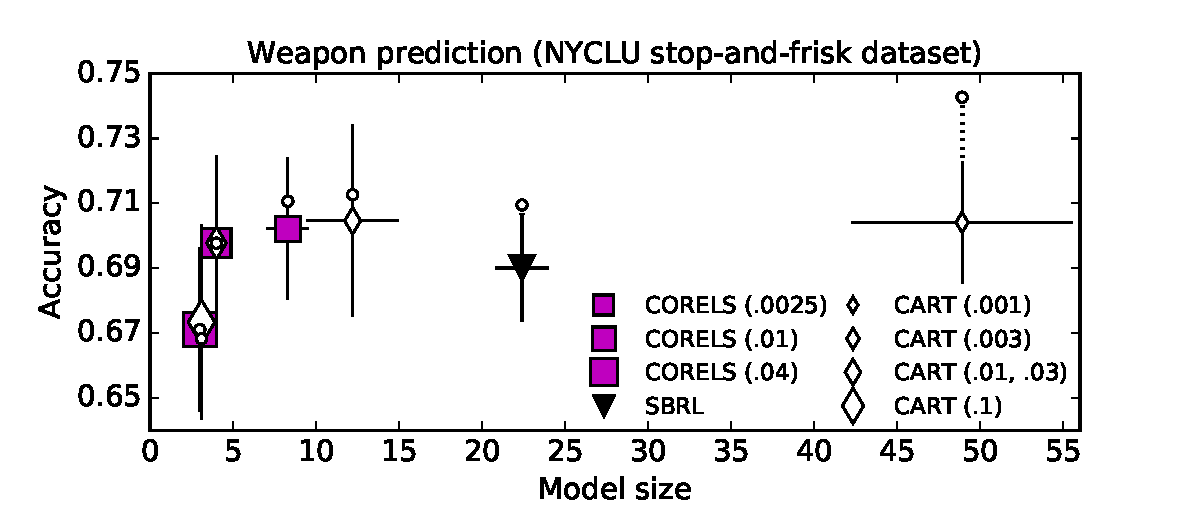
\includegraphics[trim={12mm, 5mm, 24mm, 1mm},
width=0.75\textwidth]{figs/frisk-sparsity-training.pdf}
\end{arxiv}
\begin{kdd}
% left lower right upper
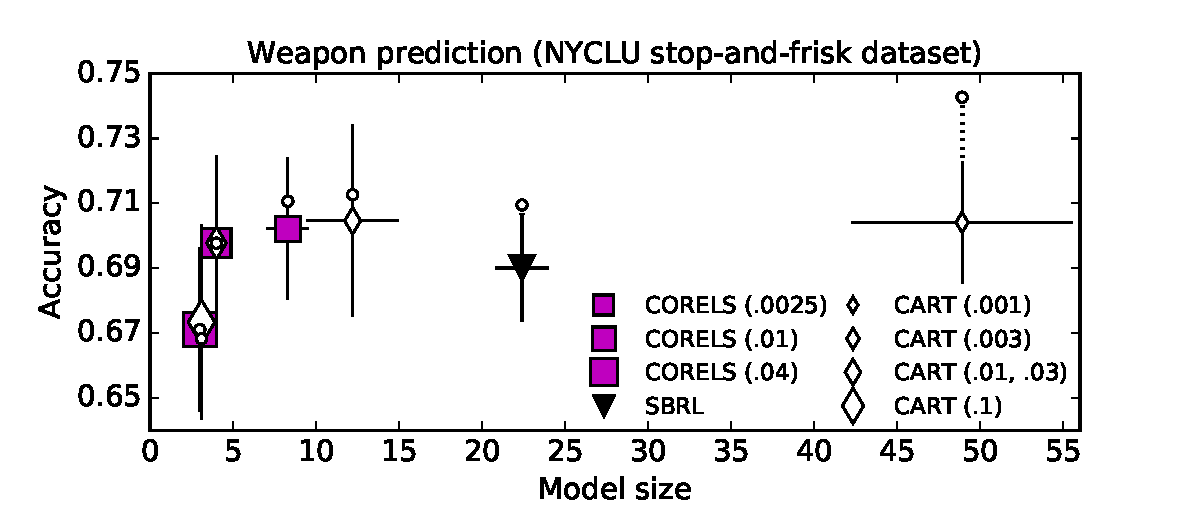
\includegraphics[trim={12mm, 12mm, 24mm, 1mm}, width=0.43\textwidth]{figs/frisk-sparsity-training.pdf}
\end{kdd}
\end{center}
\caption{Training and test accuracy as a function of model size.
%
For CORELS, CART, and C4.5, we vary the regularization parameter~$\Reg$,
and complexity parameters~$cp$ and~$C$, respectively.
% and are indicated within parentheses in the legend.
%
Legend markers and error bars indicate means and standard deviations,
respectively, of test accuracy across cross-validation folds.
%
Small circles mark associated training accuracy means.
%
Top:  %Two-year recidivism prediction for the ProPublica COMPAS dataset.
ProPublica dataset.
%
None of the models exhibit significant overfitting.
%mean training accuracy never exceeds mean test accuracy
%by more than about 0.01.
%
Bottom:  %Weapon prediction for the NYCLU stop-and-frisk dataset.
NYCLU dataset.
%
Only CART with ${cp = 0.001}$ significantly overfits.
%
We do not depict C4.5, which finds large models (${>100}$ leaves)
and dramatically overfits for all tested parameters.
}
\label{fig:sparsity}
\end{figure}

% CART implementation in R's rpart
% C4.5 = J48 in RWeka
% RIPPER in R's caret

Our experimental analysis addresses four questions:
(1) How does CORELS' accuracy and model size compare to other algorithms?
(2) How rapidly does the objective function converge?
(3) How rapidly does CORELS prune the search space?
(4) How much does each of the implementation optimizations contribute to CORELS' performance?
%
All results presented were executed on a server with two Intel Xeon E5-2699~v4
(55MB~cache, 2.20~GHz) processors and 448GB~RAM.
%
Except where we mention a memory constraint, all experiments
can run comfortably on smaller machines, \eg a laptop with 16GB~RAM.\begin{kdd}
~\footnote{Due to page constraints, we only present a subset of experiments from
an extensive evaluation contained in a long version of this report (in preparation).}
\end{kdd}
%
We focus on two problems:
using the ProPublica dataset~\cite{LarsonMaKiAn16} to predict two-year recidivism,
and using the NYCLU 2014 stop-and-frisk dataset~\cite{nyclu:2014} to predict
whether a weapon will be found on a stopped individual who is frisked or searched.

We first ran a 10-fold cross validation experiment using CORELS and eight other
algorithms:~\footnote{We use standard R packages, with default parameter settings, for the first seven.}
logistic regression, support vector machines, AdaBoost, CART, C4.5, random forests, RIPPER,~\footnote{We were unable to execute RIPPER for the NYCLU problem.} and scalable Bayesian rule lists (SBRL).~\footnote{https://github.com/Hongyuy/sbrlmod}
%
Figure~\ref{fig:rule-list} shows an  optimal rule list that CORELS learns
for the ProPublica dataset.
%
Figure~\ref{fig:comparison} shows that there were no statistically significant
differences in algorithm accuracies.
\begin{arxiv}
In fact, the difference between folds was far larger than the difference
between algorithms.
We conclude that CORELS produces models whose accuracy is comparable
to those found via other algorithms.

\end{arxiv}
%
Figure~\ref{fig:sparsity} summarizes differences in accuracy and model size
for CORELS and other tree (CART, C4.5) and rule list (RIPPER, SBRL) learning algorithms.
%
For both problems, CORELS can learn short rule lists without sacrificing accuracy.

\begin{figure}[t!]
\begin{center}
%\includegraphics[width=0.65\textwidth]{figs/sketch-objective.png}
\begin{arxiv}
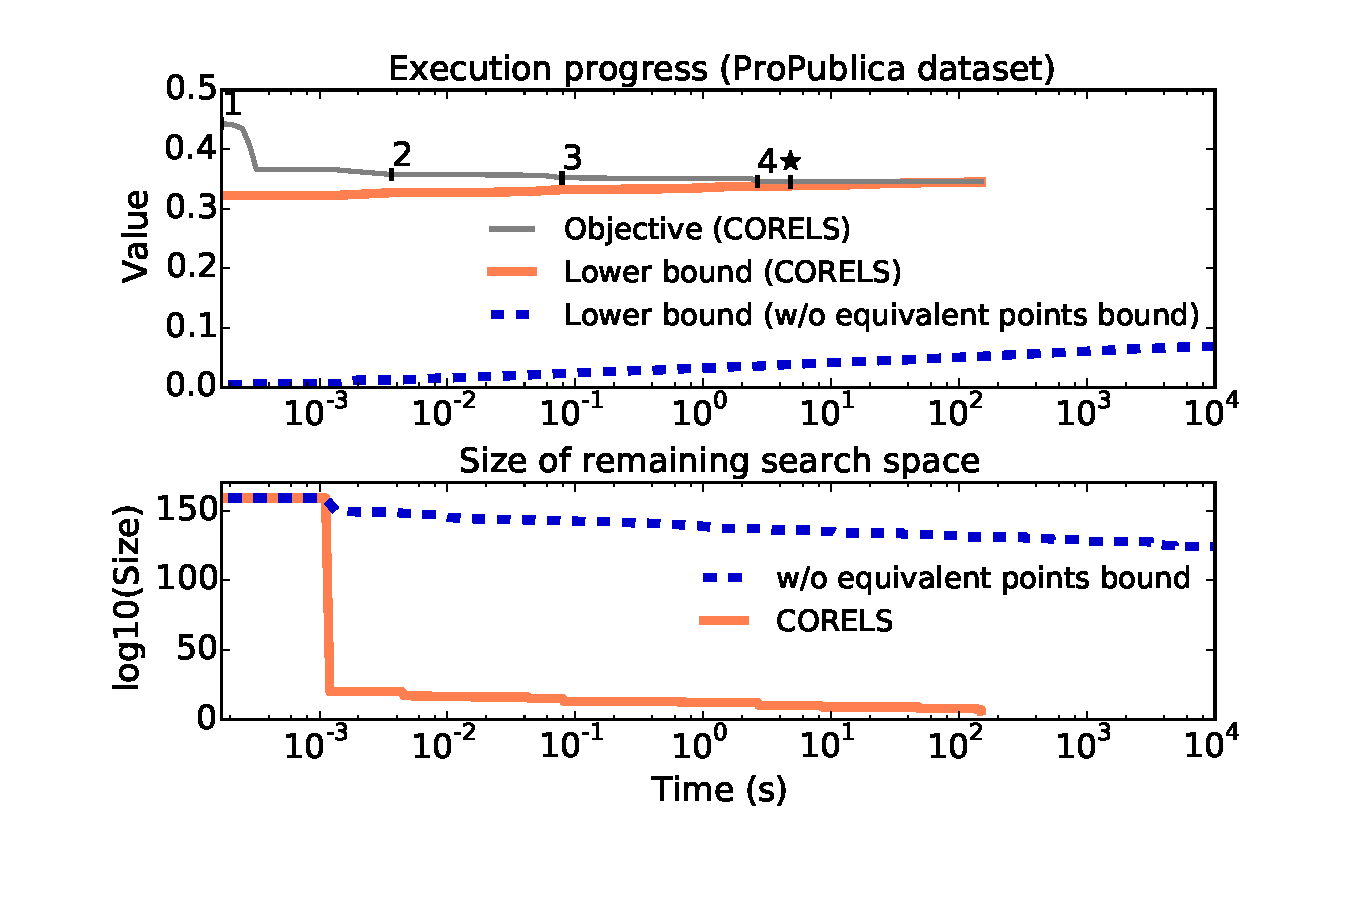
\includegraphics[trim={20mm, 15mm, 24mm, 15mm},
width=0.75\textwidth]{figs/compas_execution-remaining-space.pdf}
\end{arxiv}
\begin{kdd}
% left lower right upper
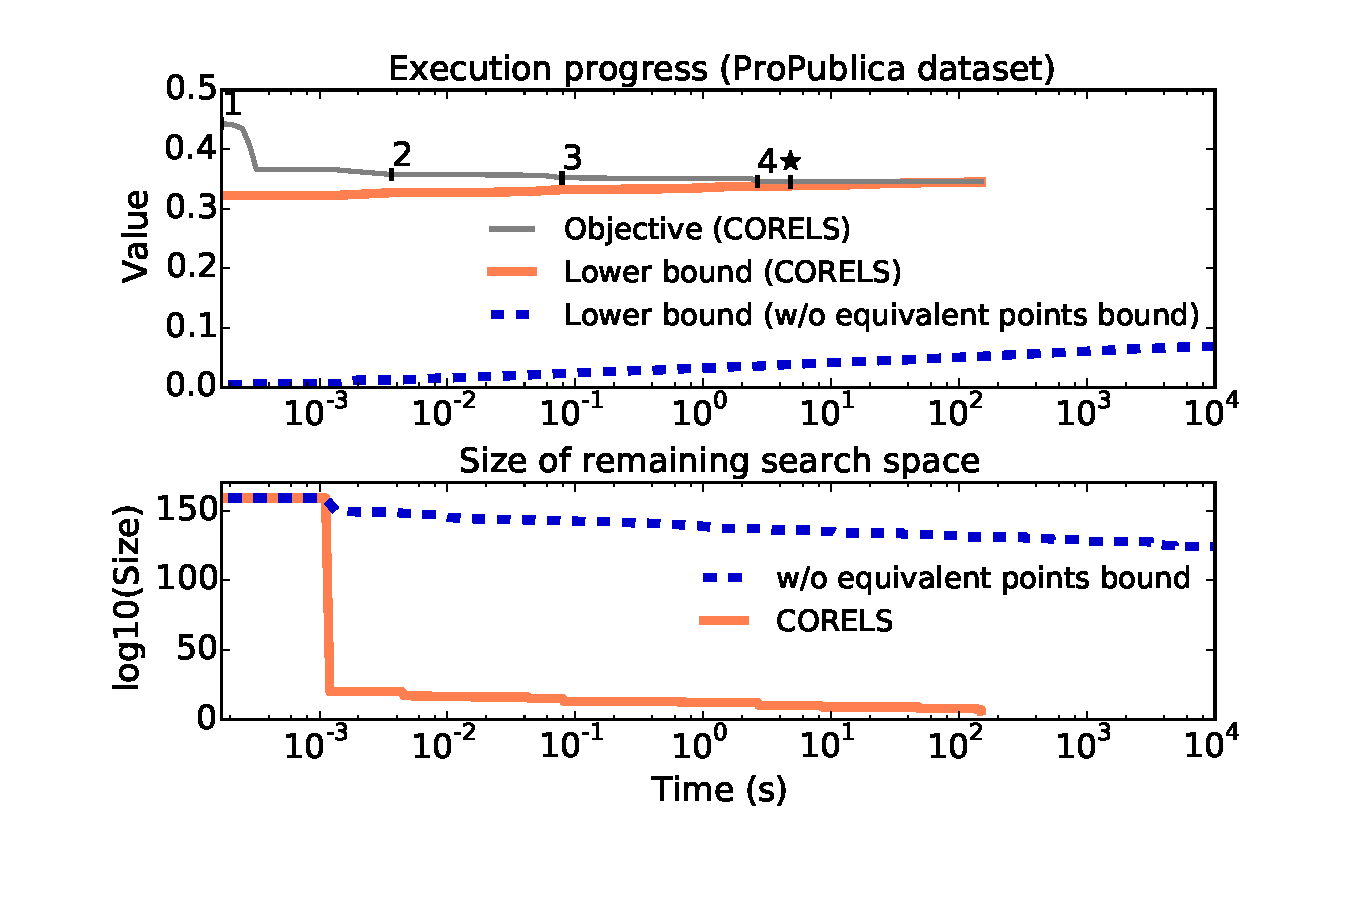
\includegraphics[trim={20mm, 25mm, 24mm, 15mm}, width=0.45\textwidth]{figs/compas_execution-remaining-space.pdf}
\end{kdd}
\end{center}
\caption{CORELS with (lines) and without
(dashes) the equivalent points bound (Theorem~\ref{thm:identical}).
%
%Horizontal axes plot wall clock time (log scale).
%
Top: Objective value (thin line) and lower bound (thick line) for CORELS,
and lower bound (dashes) for an execution without the equivalent points bound.
%as a function of wall clock time (log scale).
%
Numbered hatch marks
%along the objective
indicate when the length of the best known rule list changes,
and are labeled by the new length.
%
%CORELS quickly the optimal value (star marker),
%and certifies optimality when the lower bound matches the objective value.
A star marks the optimum.
%
% A separate execution of
%CORELS without the equivalent points bound remains far from complete,
%and its lower bound (dashed line) far from the optimum.
%
Bottom: $\lfloor \log_{10} \Remaining(\CurrentObj, \Queue) \rfloor$,
%as a function of wall clock time,
where~$\Remaining(\CurrentObj, \Queue)$
is the upper bound on remaining search space size
(Theorem~\ref{thm:remaining-eval-fine}).
}
\label{fig:objective}
\end{figure}

%\includegraphics[width=0.75\textwidth]{figs/sketch-ablation.png}
\begin{arxiv}
\begin{table}[t!]
\begin{tabular}{l | c | c | c | c | c}
Removed component & $t_\text{total}$ (min) & $t_\text{opt}$ (s) & $i_\text{total}$ ($\times 10^6$) & $Q_\text{max}$ ($\times 10^6$) & $K_\text{max}$ \\
\hline
none (CORELS) & 5.5 (1.6) & 8 (2) & 1.7 (0.4) & 1.3 (0.4) & 5-6 \\
priority queue (BFS) & 6.7 (2.2) & 4 (1) & 1.9 (0.6) & 1.5 (0.5) & 5-6 \\
support bounds & 10.2 (3.4) & 13 (4) & 2.7 (0.8) & 2.2 (0.7) & 5-6 \\
symmetry-aware map & 58.6 (23.3) & 23 (6) & 16.0 (5.9) & 14.5 (5.7) & 5-6 \\
lookahead bound & 71.9 (23.0) & 9 (2) & 18.5 (5.9) & 16.3 (5.3) & 6-7 \\
%equiv. pts. bound & 188.6 (104.6) & 6178 (1840) & 803.8 (0.1) & 790.5 (0.4) & 10-10
equivalent pts bound & $>$134 & $>$7168* & $>$800 & $>$789 & $\ge$10
\end{tabular}
\vspace{4mm}
\caption{Per-component performance improvement.
%
The columns report total execution time,
time to optimum, number of queue insertions,
maximum queue size, and maximum evaluated prefix length.
%
The first row shows CORELS; subsequent rows show variants
that each remove a specific implementation optimization or bound.
%
(We are not measuring the cumulative effects of removing a sequence of components.)
%
All rows represent complete executions, except for the final row,
in which each execution was terminated due to memory constraints,
once the size of the cache reached ${8 \times 10^8}$ elements,
after consuming 390-410GB RAM.
We terminated each experiment in the last row after consuming 390-410GB RAM.
%
In all but the final row and column, we report means
(and standard deviations) over 10 cross-validation folds;
in the final row, we report the minimum values across folds. \\
%
*~Only 4 out of 10 folds achieve the optimum before being terminated.
}
\label{tab:ablation}
\end{table}
\end{arxiv}
\begin{kdd}
\begin{table}[t!]
\centering
\resizebox{0.49\textwidth}{!}{
\begin{tabular}{l | c | c | c | c | c}
Removed & $t_\text{total}$ & $t_\text{opt}$ & $i_\text{total}$ & $Q_\text{max}$ & $K_\text{max}$ \\
component & (min) & (s) & ($\times 10^6$) & ($\times 10^6$) & \\
\hline
none (CORELS) & 5.5 (1.6) & 8 (2) & 1.7 (0.4) & 1.3 (0.4) & 5-6 \\
priority queue (BFS) & 6.7 (2.2) & 4 (1) & 1.9 (0.6) & 1.5 (0.5) & 5-6 \\
support bounds & 10.2 (3.4) & 13 (4) & 2.7 (0.8) & 2.2 (0.7) & 5-6 \\
symmetry-aware map & 58.6 (23.3) & 23 (6) & 16.0 (5.9) & 14.5 (5.7) & 5-6 \\
lookahead bound & 71.9 (23.0) & 9 (2) & 18.5 (5.9) & 16.3 (5.3) & 6-7 \\
%equiv. pts. bound & 188.6 (104.6) & 6178 (1840) & 803.8 (0.1) & 790.5 (0.4) & 10-10
equivalent pts bound & $>$134 & $>$7168 & $>$800 & $>$789 & $\ge$10
\end{tabular}
}
\vspace{4mm}
\caption{Per-component performance improvement.
%
The columns report total execution time,
time to optimum, number of queue insertions,
maximum queue size, and maximum evaluated prefix length.
%
The first row shows CORELS; subsequent rows show variants
that each remove a specific implementation optimization or bound.
%
We terminated each experiment in the last row after consuming 390-410GB RAM.
%
In all but the final row and column, we report means
(and standard deviations) over 10 cross-validation folds;
in the final row, we report the minimum values across folds.
}
\label{tab:ablation}
\vspace{-8mm}
\end{table}
\end{kdd}

In the remainder, we show results using the ProPublica dataset.
%
Figure~\ref{fig:objective} illustrates how both the objective and the size of
the remaining search space decrease as CORELS executes.
The objective drops quickly, achieving the optimal value within 10 seconds.
CORELS certifies optimality in less than 6 minutes --
the objective lower bound of the remaining search space
steadily converges to the optimal objective as the search space shrinks.

Finally, we determine the efficacy of each of our bounds and data structure optimizations.
%
Figure~\ref{fig:objective} highlights how a separate execution of CORELS without
the equivalent points bound remains far from complete,
with its lower bound far from the optimum.
%
Table~\ref{tab:ablation} provides summary statistics for experiments using
the full CORELS implementation and variants each remove a specific optimization.
%
Figure~\ref{fig:queue} presents a view of the same experiments, focusing
on three of our optimizations. These plots depict the number of
prefixes of a given length in the queue during the algorithm's execution.

\begin{arxiv}
\begin{figure}[t!]
\begin{center}
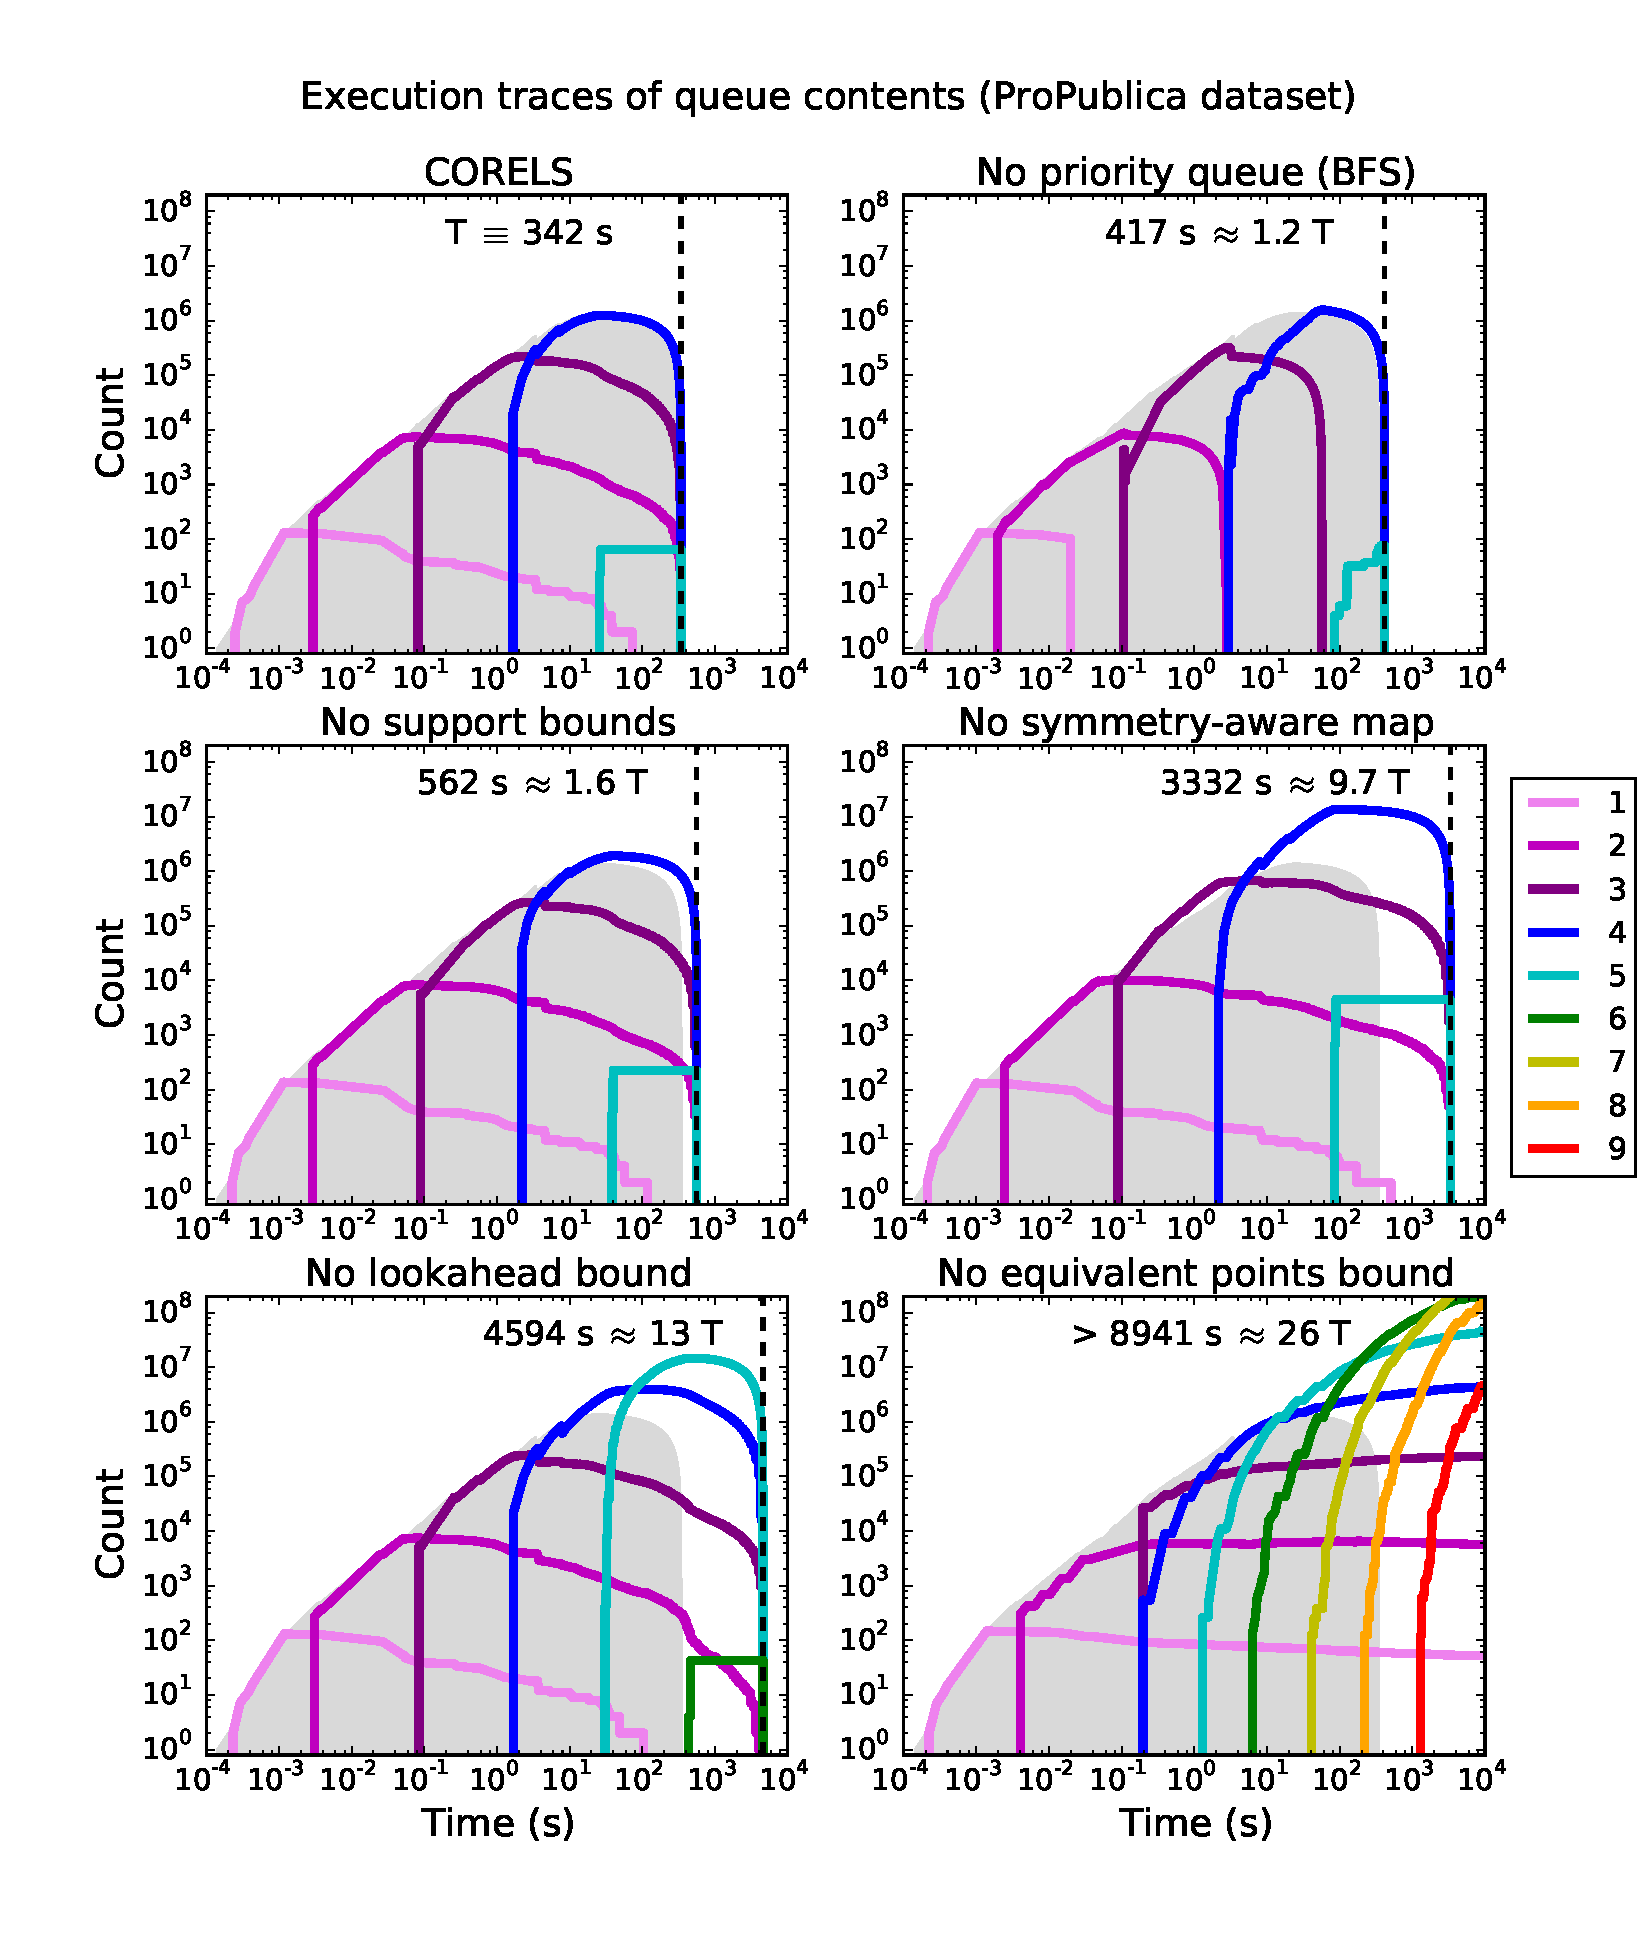
\includegraphics[trim={30mm 10mm 35mm 30mm},
width=\textwidth]{figs/kdd_compas_ablation-queue.pdf}
\end{center}
\caption{Logical queue composition.
%
Numbers of prefixes in the queue (log scale), labeled and colored by length,
as a function of wall clock time (log scale), for CORELS (top left),
and without five specific implementation optimizations or bounds.
%the permutation bounds (top right),
%lookahead bound (bottom left), and equivalent points bound (bottom right).
%
The gray shading fills in the area beneath the total number of
queue elements for CORELS.
\ie the sum over all lengths in the top left figure.
%
For comparison, we replicate the same gray region
in the other three subfigures.
}
\label{fig:queue}
\end{figure}
\end{arxiv}
\begin{kdd}
\begin{figure}[t!]
\begin{center}
% left lower right upper
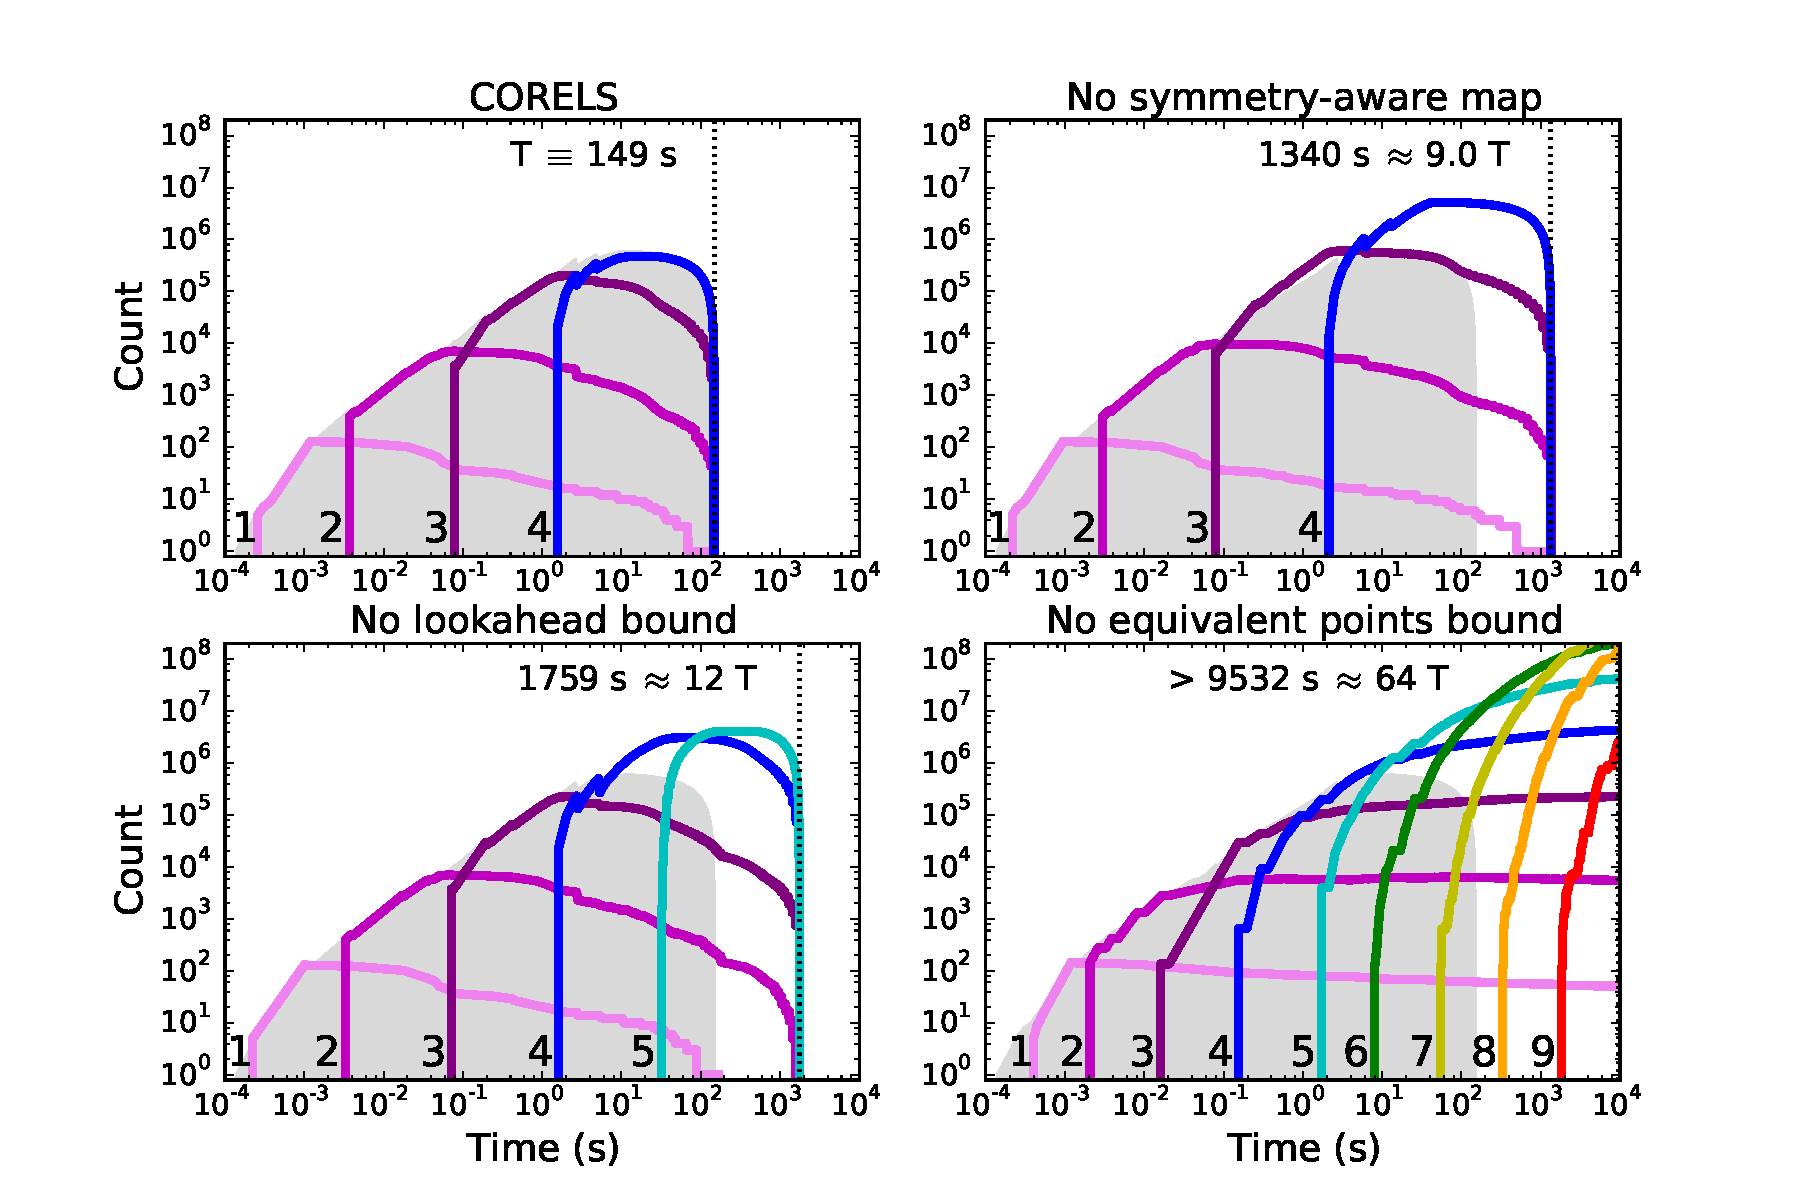
\includegraphics[trim={30mm 15mm 35mm 30mm},
width=0.45\textwidth]{figs/kdd_compas_ablation_small-queue.pdf}
\end{center}
\caption{Queue composition.
%
Numbers of prefixes in the queue (log scale), labeled and colored by length,
as a function of wall clock time (log scale), for CORELS (top left),
and without three specific implementation optimizations or bounds.
%
The gray shading fills in the area beneath the total number of
queue elements for CORELS.
\ie the sum over all lengths in the top left figure.
%
For comparison, we replicate the same gray region
in the other three subfigures.
}
\label{fig:queue}
\end{figure}
\end{kdd}

\begin{comment}

\begin{table}[t!]
\centering
\begin{tabular}{l | c | c}
Method & ProPublica & NYCLU \\
\hline
CORELS & 67.6 $\pm$ 2.0 & 69.8 $\pm$ 2.7 \\
SBRL & 67.1 $\pm$ 1.7 & 69.7 $\pm$ 2.0 \\
CART & 66.7 $\pm$ 2.1 & 69.8 $\pm$ 2.7 \\
C4.5 & 67.3 $\pm$ 1.8 & 66.8 $\pm$ 2.1 \\
RF & 67.3 $\pm$ 1.8 & 68.7 $\pm$ 2.4 \\
RIPPER & 67.3 $\pm$ 2.0 & --- \\
AdaBoost & 67.3 $\pm$ 1.7 & 70.6 $\pm$ 2.7 \\
GLM & 67.5 $\pm$ 1.8 & 70.3 $\pm$ 2.5 \\
SVM & 67.1 $\pm$ 2.0 & 70.2 $\pm$ 2.7 \\
\end{tabular}
\vspace{5mm}
\caption{Comparison with other methods:
Means and standard deviations of test accuracy.
Also report algorithm runtimes (mean $\pm$ standard deviation over 10 folds).
CORELS ${\Reg = 0.005}$ for ProPublica and ${\Reg = 0.01}$ for NYCLU.}
\label{tab:comparison}
\end{table}

\begin{figure}[t!]
\begin{center}
\end{center}
\caption{Missing:  Some sort of comparison of different scheduling policies}
\label{fig:scheduling-policy}
\end{figure}

\begin{figure}[t!]
\begin{center}
%\includegraphics[width=0.65\textwidth]{figs/sketch-queue-size.png}
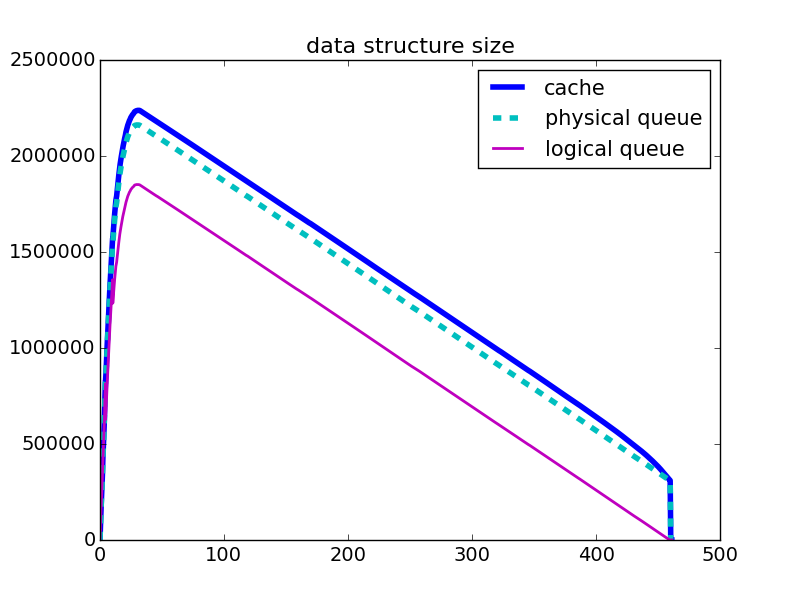
\includegraphics[width=0.8\textwidth]{figs/ela_compas-queue-cache-size-insertions.pdf}
\end{center}
\caption{Cache and queue data structure sizes and insertions.
%
The top plot shows the sizes of the cache and queue data structures,
as a function of wall clock time.
%
The number of nodes in the cache (solid black line) is an
upper bound on the number of elements in the physical queue
(dotted gray line), since the physical queue elements only
correspond to the cache trie data structure's leaf nodes
plus disconnected cache nodes that have been marked for deletion.
%
The queue's physical size is an upper bound on its
logical size (solid blue line), which doesn't include nodes
that have been marked for deletion.
%
The bottom plot shows the cumulative number of cache insertions,
which is equivalent to the cumulative number of queue insertions,
as a function of wall clock time.
}
\label{fig:queue-cache-size-insertions}
\end{figure}

\begin{figure}[t!]
\begin{center}
%\includegraphics[width=0.65\textwidth]{figs/sketch-max-length.png}
\includegraphics[width=0.8\textwidth]{figs/ela-max-length-check.png}
\end{center}
\caption{Max prefix length over time (computed from objective value)}
\label{fig:max-length}
\end{figure}

\begin{figure}[t!]
\begin{center}
\includegraphics[width=0.8\textwidth]{figs/ela_compas-prefix-length.pdf}
\end{center}
\caption{Best prefix length over time}
\label{fig:prefix-length}
\end{figure}
\end{comment}
